\setchapterstyle{kao}
\setchapterpreamble[u]{\margintoc}

\chapter{Standard Model Neutrinos}
\labch{sm_neutrinos_properties}


\todo{(Re-)write SM neutrino chapter for PhD thesis (just copy paste from M.Sc.).}


This chapter introduces the basic properties of neutrinos, their place in the Standard Model of particle physics (SM) and their peculiarities following the description of \sidecite{Thomson_Particle}.
Section \refsec{neutrino_properties} and Section \refsec{neutrino_interactions} state the general properties of neutrinos and the neutrino-nucleon interactions.
After describing atmospheric neutrinos in Section \refsec{neutrino_atmospheric} the phenomenon of neutrino oscillations is presented in Section \refsec{neutrino_oscillations}.



\section{Standard Model Particles}

\subsection{Electroweak Symmetry Breaking}

\subsection{Charged Fermion Masses}

\subsection{Neutrino Masses}

\subsubsection{Dirac}

\subsubsection{Majorana}


\subsection{See-Saw Mechanisms}

\subsection{Radiative Neutrino Masses}


\section{Neutrino Properties}

\subsection{Quantum Numbers}

\subsection{Mass}

\subsection{Active Neutrino Flavors}


\section{Neutrino Interactions} \labsec{neutrino_interactions}

\subsection{Weak Interactions after Symmetry-Breaking}

The neutrino is an elementary particle in the SM \sidecite{Thomson_Particle}.
It belongs to the class of leptons, which itself is a subclass of elementary fermions (spin ${\frac{1}{2}}$ particles).
The fermions - six quarks and six leptons - form the matter content of the universe.
Quarks take part in all three interaction types (forces) of the SM: strong, weak, and electromagnetic (EM) \sidecite{GLASHOW1961579}.
The charged leptons - electron, muon, and tau - are subject to the weak and the EM interaction.
Neutrinos carry neither electric charge nor color charge and therefore only take part in weak interactions.
There are three distinct neutrino flavors - electron neutrinos, muon neutrinos and tau neutrinos ($\nu_e$, $\nu_{\mu}$, and $\nu_{\tau}$) \sidecite{PhysRevD.98.030001} - each corresponding to their charged lepton counterparts.

\begin{figure}
	\centering
    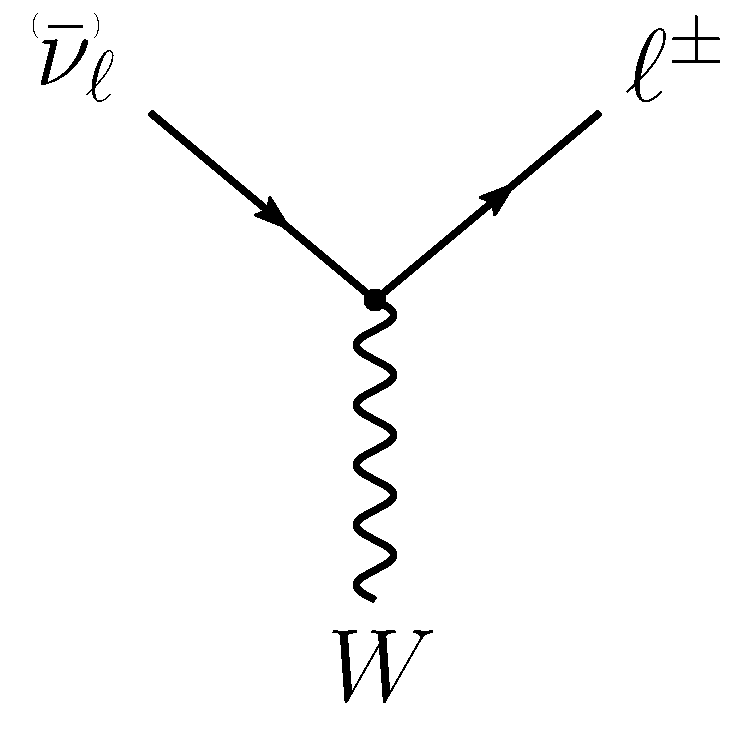
\includegraphics[width=0.25\linewidth]{figures/neutrinos_properties/feynman_CC_nu.pdf}
    \hspace{1cm}
    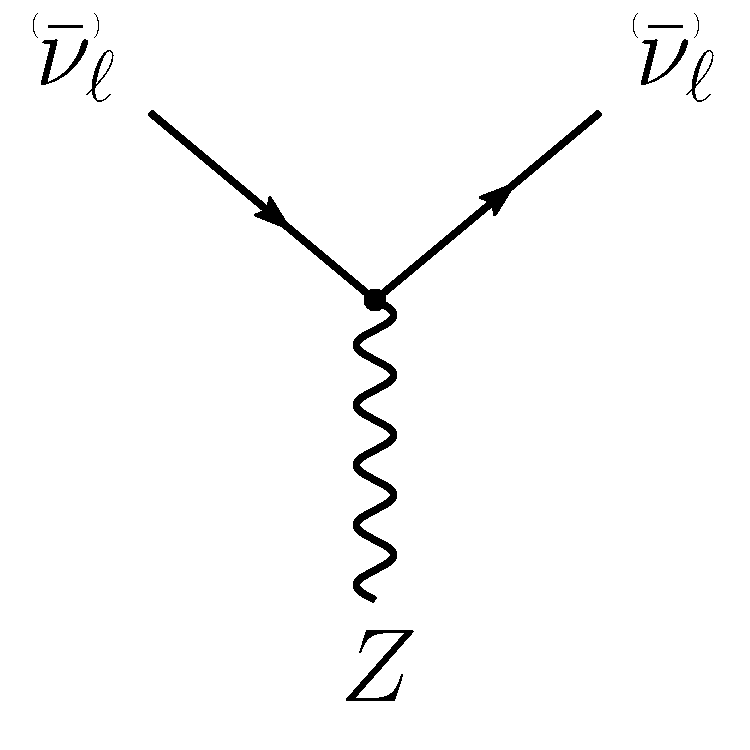
\includegraphics[width=0.25\linewidth]{figures/neutrinos_properties/feynman_NC_nu.pdf}
    \caption[Feynman diagrams of neutrino weak interactions, taken from \cite{ATerliuk}]
    {Feynman diagrams of charged-current (left) and neutral-current (right) neutrino weak interactions. Taken from \cite{ATerliuk}.}
    \label{fig:weak_interactions}
\end{figure}

In the SM, weak interactions are mediated by the three massive bosons $\textbf{W}^+$, $\textbf{W}^-$, and $\textbf{Z}^0$ \sidecite{Thomson_Particle}.
The large boson masses ($m_{\textbf{W}}\sim80$\,GeV, $m_{\textbf{Z}}\sim90$\,GeV) result in a short range of the force of about $10^{-18}$\,m.
Weak interactions carried by $\textbf{W}^\pm$ bosons are called charged-current (CC) interactions, because charge is transferred between the interacting particles.
In CC interactions, a neutrino is converted into its corresponding charged lepton or vice versa.
Neutral current (NC) interactions are those mediated by $\textbf{Z}^0$ bosons.
Here no charge is transferred.
The Feynman diagrams for CC and NC interactions are shown in Figure \reffig{weak_interactions}.

Although neutrinos are massless in the SM, we know today that they do have a small mass.
The observed phenomenon of neutrino oscillations (see Section \refsec{neutrino_oscillations}) is based on the fact that there is a mass difference between the three neutrino mass eigenstates.
From neutrino oscillation measurements the absolute mass scale cannot be determined, since they only depend on the mass differences, but there are upper limits on the sum of all neutrino masses from cosmological observations.
These upper limits are typically between $0.3$ and $1.3$\,eV \sidecite{PhysRevD.98.030001}.


\subsection{Neutrino-Lepton Scattering}

\subsubsection{Particle-Antiparticle Scattering}


\subsection{Neutrino Interactions with Nuclei}

To describe the neutrino detection principle of IceCube explained in Chapter \refch{icecube} we need to understand the weak interaction processes that occur at the energies relevant for this work ($10-100$\,GeV).
The cross-sections are dominated by the following neutrino-nucleon interactions: quasi-elastic scattering (QE), resonant scattering (RES), and deep inelastic scattering (DIS).
The relative importance of the different processes depends on energy as can be seen in Figure \reffig{cross_sections}.

\begin{figure}[ht]
	\centering
    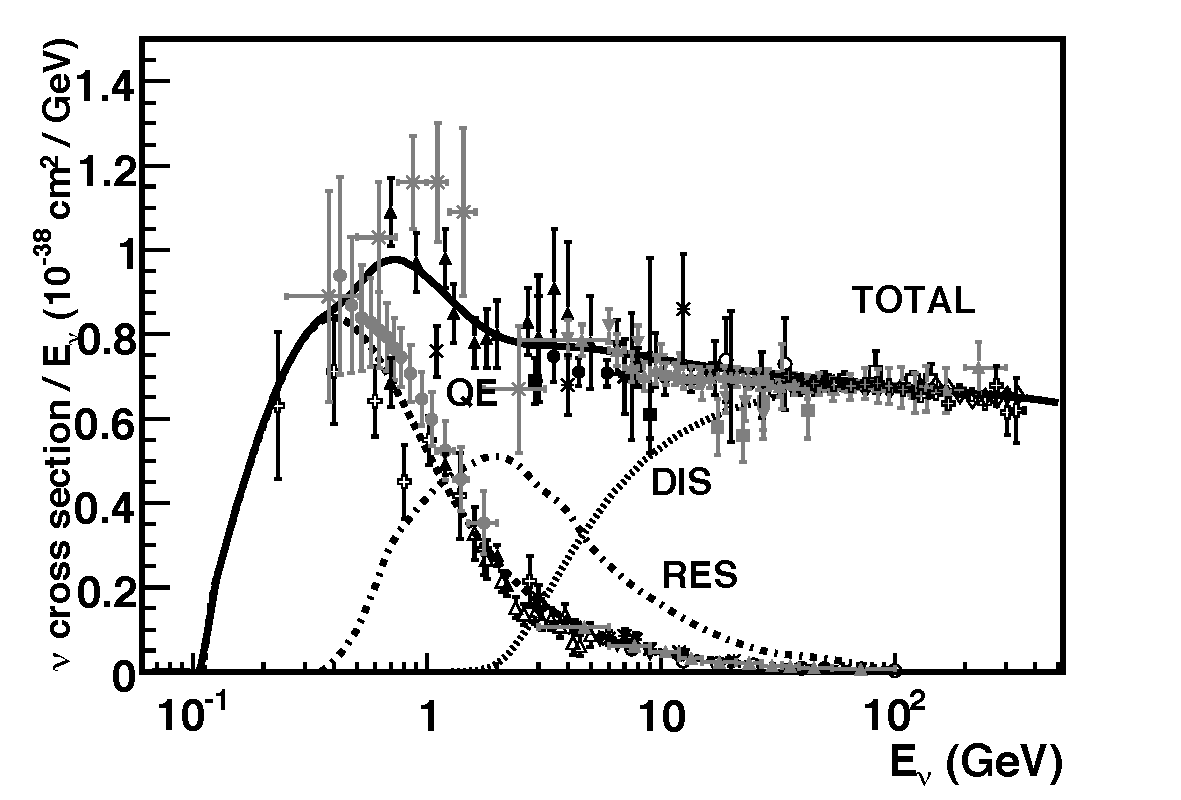
\includegraphics[width=0.495\linewidth]{figures/neutrinos_properties/cc_inclusive_nu.pdf}
    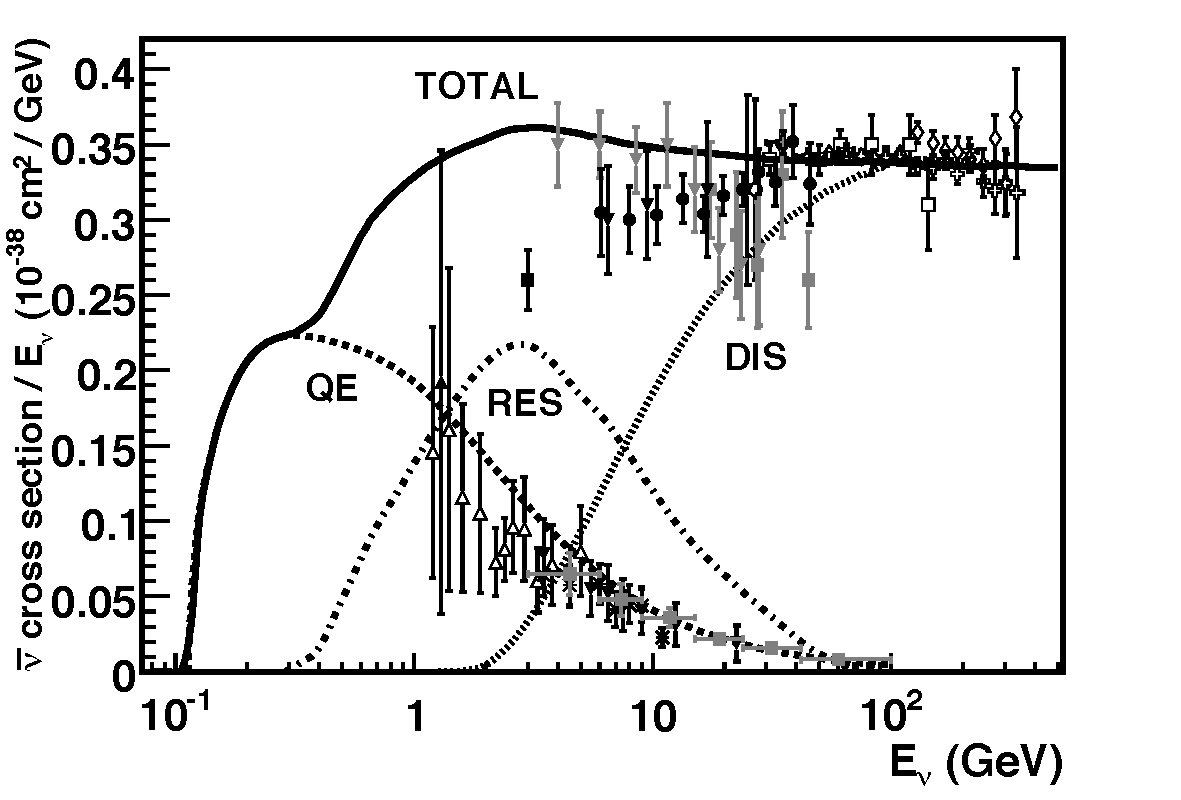
\includegraphics[width=0.495\linewidth]{figures/neutrinos_properties/cc_inclusive_nubar.pdf}
	\caption[Total inclusive neutrino-nucleon cross-sections, taken from \cite{Formaggio_Cross_Sections}.]{Total neutrino(left) and antineutrino(right) per nucleon cross-section divided by neutrino energy plotted against energy.
    The three main scattering processes quasi-elastic scattering (QE), resonant scattering (RES), and deep-inelastic scattering (DIS) are depicted. Taken from \cite{Formaggio_Cross_Sections}.}
    \labfig{cross_sections}
\end{figure}

An extensive description of all the interactions and the differences between neutrino and antineutrino cross-sections can be found in \sidecite{Formaggio_Cross_Sections}.
At energies below 5\,GeV, QE and RES occur and the neutrinos interact with approximately point-like protons and neutrons.
The cross-sections of these processes are not linear in energy and the transition region to higher energies is poorly understood.
At higher energies, the interactions are dominated solely by DIS which has a linear dependence on energy above $\sim20\,$GeV.
For a given neutrino energy, it is possible to predict the cross-section in this region.
Here neutrinos interact with a single quark, breaking apart the nucleus and producing a shower of relativistic secondary particles.
Neutrino DIS is the primary detection channel of IceCube.
From Figure \reffig{cross_sections} it can be seen that the interaction cross-sections are very small of the order of $10^{-38}\mathrm{\,cm}^2$.
Because of the small interaction cross-section, very large volume detectors are required to capture a sufficiently large sample of neutrinos to use for precision studies of their properties.
For example, the interaction length of a neutrino with $E_\nu = 10$\,GeV is of $\mathcal{O}(10^{10}\,\mathrm{km})$.


\subsubsection{Charged-current Quasi-elastic Scattering}

\paragraph{Quasi-elastic scattering (QE)} with nucleons is the main process below 1\,GeV.
Protons are converted to neutrons in antineutrino interactions and vice-versa for neutrino interactions.
Additionally, a charged lepton corresponding to the neutrino/antineutrino flavor is produced.


\subsubsection{Resonant Scattering}

\paragraph{Resonant scattering (RES)} describes the process of a neutrino scattering off a nucleon producing an excited state of the nucleon in addition to a charged lepton.
RES is the leading process at 1.5-5\,GeV for neutrinos and 1.5-8\,GeV for antineutrinos.


\subsubsection{Deep Inelastic Scattering}

\paragraph{Deep inelastic scattering (DIS)} occurs if a neutrino carries sufficient energy to resolve the underlying structure of the nucleon and interacts with one of the composing quarks.
DIS is the dominant process above 10\,GeV. The nucleon breaks up and a lepton accompanied by a set of hadronic final states is produced.
Whether the lepton is the charged lepton corresponding to the interacting neutrino type, or the neutrino itself depends on the type of DIS interaction.
DIS happens via CC as in 
\begin{equation}
    \begin{split}
        \nu_l + N \rightarrow l^- + X, \\
        \bar{\nu}_l + N \rightarrow l^+ + X, \\
    \end{split}
    \labeq{dis_cc}
\end{equation}
or NC interactions as
\begin{equation}
    \nu_l + N \rightarrow \nu_l + X.
        \labeq{dis_nc}
\end{equation}
Here, $X$ stands for any set of final state hadrons and $N$ for the nucleon.
The Feynman diagrams for the processes in Equations \refeq{dis_cc} and \refeq{dis_nc} are shown in Figure \reffig{dis_feynman}.

\begin{figure}[h]
    \centering
    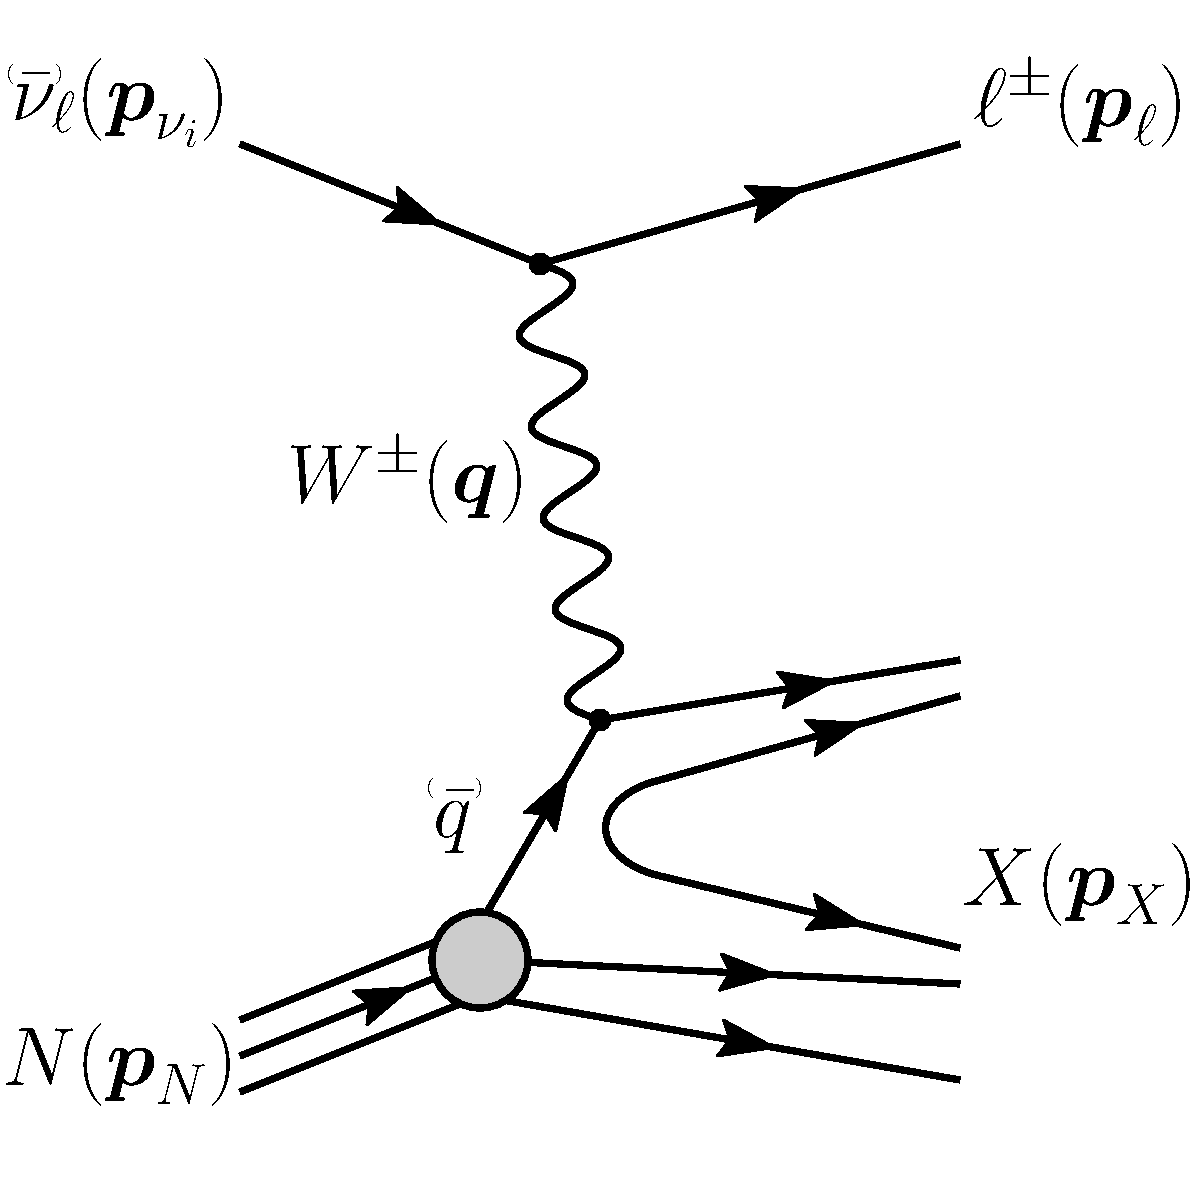
\includegraphics[width=0.4\linewidth]{figures/neutrinos_properties/feynman_DIS_CC_nu_new.pdf}
    \hspace{0.8cm}
    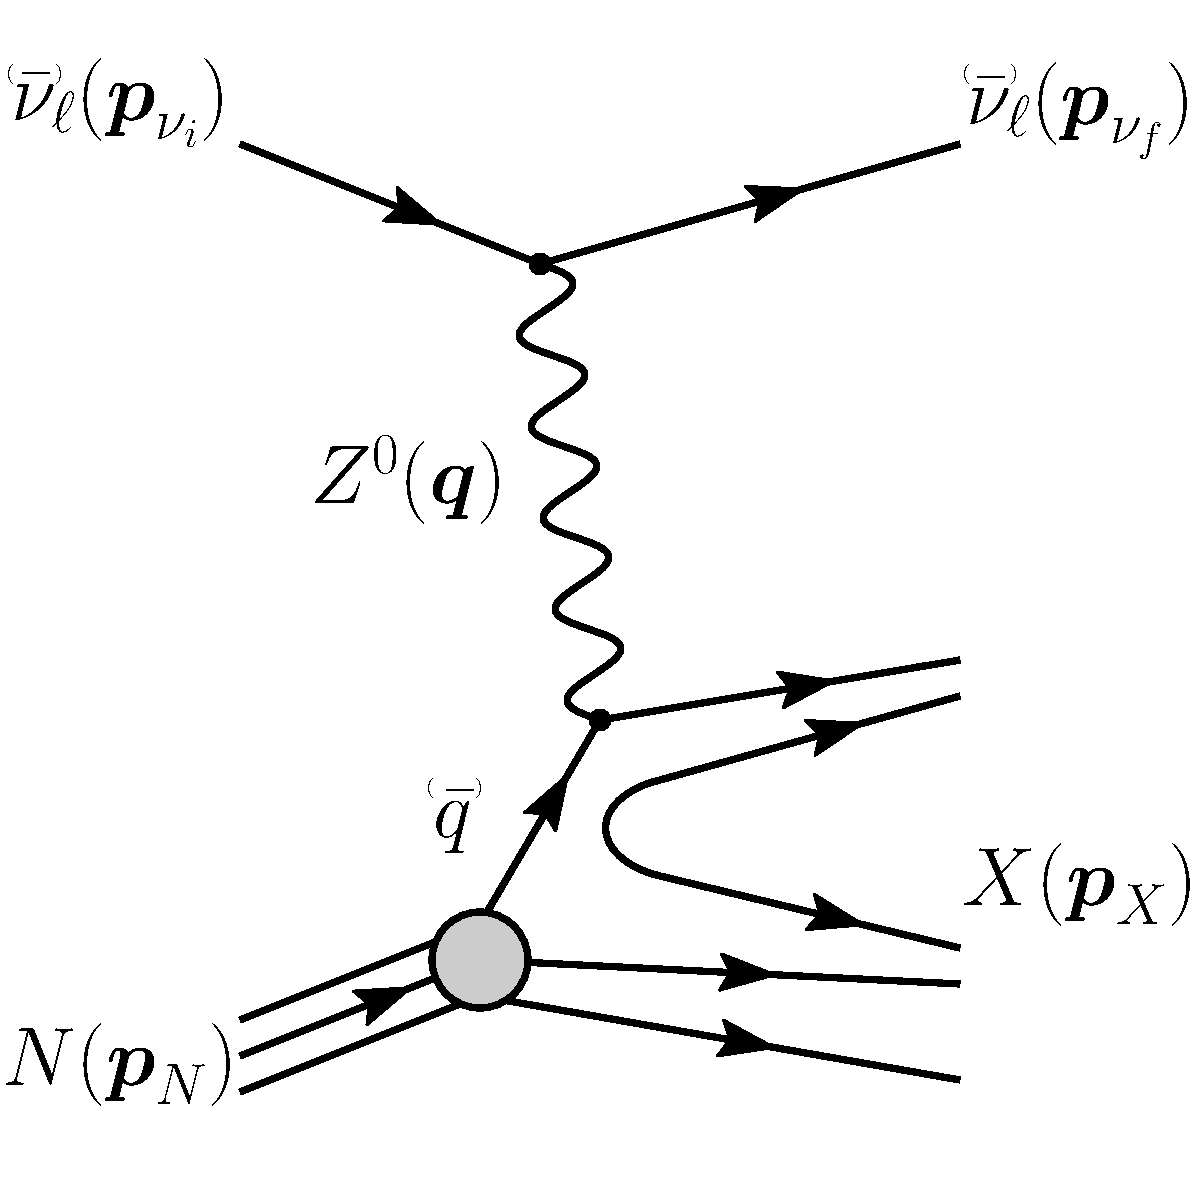
\includegraphics[width=0.4\linewidth]{figures/neutrinos_properties/feynman_DIS_NC_nu_new.pdf}
    \caption[Neutrino-nucleon deep inelastic scattering, taken from \cite{ATerliuk}]{Feynman diagrams for deep inelastic scattering of a neutrino with a nucleon via charged-current (left) and neutral current (right) interactions. Taken from \cite{ATerliuk}.}
    \labfig{dis_feynman}
\end{figure}
